\newsection{Advanced}

\underline{\textlg{\textbf{Questions are continued on the next page}}}
\newpage
\begin{enumerate}
%======================================================
\item \textlg{\textbf{Given an array of integers, can you rotate them k steps to the right?}}

%QUESTION SPECIFICS/IMAGES HERE

%EXAMPLES HERE
\begin{console}
Example 1: [1,2,3,4,5,6,7], k = 3
Output:    [5,6,7,1,2,3,4]

Explanation:
rotate 1 steps to the right: [7,1,2,3,4,5,6] 
rotate 2 steps to the right: [6,7,1,2,3,4,5] 
rotate 3 steps to the right: [5,6,7,1,2,3,4]

Example 2: [-1,-100,3,99], k = 2
Output:    [3,99,-1,-100]

Explanation:
rotate 1 steps to the right: [99,-1,-100,3]
rotate 2 steps to the right: [3,99,-1,-100]

\end{console}
\newpage


%======================================================
\item \textlg{\textbf{Given a signed 32-bit integer x, return x with its digits reversed.}}

%QUESTION SPECIFICS/IMAGES HERE
If reversing x causes the value to go outside the signed 32-bit integer range [$-2^{31}$,  $2^{31 - 1}$], then return 0.

64-bit integers (signed or unsigned) are not allowed.

%EXAMPLES HERE
\begin{console}
Example 1: 123 
Output:    321 

Example 2: -123 
Output:    -321 

Example 3: 120 
Output:    21
\end{console}
\newpage


%======================================================
\item \textlg{\textbf{Given two non-negative integers num1 and num2 represented as strings, return the product of num1 and num2, also represented as a string.}}

%QUESTION SPECIFICS/IMAGES HERE
Note: You must not use any built-in BigInteger library or convert the inputs to integers directly. 

%EXAMPLES HERE
\begin{console}
Example 1: num1 = "2", num2 = "3" 
Output:    "6" 

Example 2: num1 = "123", num2 = "456"
Output:    "56088"
\end{console}
\newpage


%======================================================
\item \textlg{\textbf{Given a string of words, reverse their order of appearance.}}

%QUESTION SPECIFICS/IMAGES HERE
Remove all leading / trailing whitespace
%EXAMPLES HERE
\begin{console}
Example: "the sky is blue" 
Output:  "blue is sky the"

Example: "  hello world  " 
Output:  "world hello" 
\end{console}
\newpage


%======================================================
\item \textlg{\textbf{Given a list of numbers, determine exactly how many numbers are strictly smaller than the current number for every single element in the list.}}

%QUESTION SPECIFICS/IMAGES HERE
Count all the strictly smaller values across the entire list and return these counts in a new list that corresponds to the exact order of the original numbers.

%EXAMPLES HERE
\begin{console}
Example 1: [8,1,2,2,3] 
Output:    [4,0,1,1,3]
\end{console}
\newpage


%======================================================
\item \textlg{\textbf{Imagine a black-and-white image represented as a 2D grid of 0s and 1s. You need to apply two transformations to this grid in order.}}

%QUESTION SPECIFICS/IMAGES HERE
First, flip the image horizontally, meaning the elements of each row are reversed. Then, invert the image, meaning every 0 becomes a 1 and every 1 becomes a 0. Return the final transformed grid.

%EXAMPLES HERE
\begin{console}
Example 1: [[1,1,0],[1,0,1],[0,0,0]] 
Output:    [[1,0,0],[0,1,0],[1,1,1]]
\end{console}
\newpage


%======================================================
\item \textlg{\textbf{You are given a main text string and a target substring. You need to continuously search for the leftmost appearance of the target substring within the main text and delete it.}}

%QUESTION SPECIFICS/IMAGES HERE
After deleting a substring, the remaining pieces of the main text will slide together, which might form a brand new occurrence of the target. Continue this deletion process until the target substring can no longer be found anywhere, and return the final string.

%EXAMPLES HERE
\begin{console}
Example 1: "daabcbaabcbc", target = "abc" 
Output:    "dab"
\end{console}
\newpage


%======================================================
\item \textlg{\textbf{You are given a list of words. Filter this list and return only the words that can be typed using just a single row of a standard English QWERTY keyboard.}}

%QUESTION SPECIFICS/IMAGES HERE
For reference, the top row is "qwertyuiop", the middle row is "asdfghjkl", and the bottom row is "zxcvbnm". Your logic should be completely unaffected by uppercase or lowercase letters.

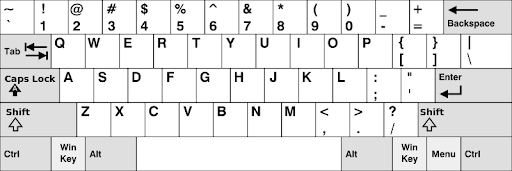
\includegraphics[scale=0.45]{images/keyboard.png}

%EXAMPLES HERE
\begin{console}
Example 1: ["Hello","Alaska","Dad","Peace"]
Output:    ["Alaska","Dad"]
\end{console}
\newpage



%======================================================
\item \textlg{\textbf{Given an array of positive numbers and a target divisor, find the length of the shortest contiguous subarray that you can remove so that the sum of the remaining elements is perfectly divisible by the target divisor.}}

%QUESTION SPECIFICS/IMAGES HERE
If it is already divisible, you remove nothing. If it is impossible to achieve this, or if you would need to remove the entire array to make it work, consider it a failure and return -1.

%EXAMPLES HERE
\begin{console}
Example 1: [3,1,4,2], divisor = 6 
Output:    [1]
\end{console}
\newpage



%======================================================
\item \textlg{\textbf{You are given an integer and must convert it into its Roman numeral equivalent.}}

%QUESTION SPECIFICS/IMAGES HERE
Roman numerals are represented by seven different symbols: I (1), V (5), X (10), L (50), C (100), D (500), and M (1000). They are typically written from largest to smallest, left to right. However, there are subtractive exceptions for 4 (IV), 9 (IX), 40 (XL), 90 (XC), 400 (CD), and 900 (CM).

%EXAMPLES HERE
\begin{console}
Example 1: 58 
Output:    "LVIII"
\end{console}
\newpage


%======================================================
\item \textlg{\textbf{Given an integer array nums, move all 0's to the end of it while maintaining the relative order of the non-zero elements.}}

%QUESTION SPECIFICS/IMAGES HERE
Note that you must do this in-place without making a copy of the array.

%EXAMPLES HERE
\begin{console}
Example 1: [0,1,0,3,12]
Output:    [1,3,12,0,0]
\end{console}
\newpage


%======================================================
\item \textlg{\textbf{You are given a string that contains regular letters and star symbols ('*').}}
%\newcounter{qc}
%QUESTION SPECIFICS/IMAGES HERE
Whenever you encounter a star in the text, you must remove the star itself along with the closest non-star character immediately to its left. Process the text and return the final string after all stars have been applied and removed.

%EXAMPLES HERE
\begin{console}
Example 1: "hello wo**rld" 
Output:    "hello rld"

Example 2: "what*s up"
Output:    "whas up"
\end{console}
\newpage
 

\end{enumerate}

\newpage
For this section, you should know your data structures and algorithms. If you don't, feel free to look anyways, but keep in mind these questions are very challenging even to those who do know their DSA.\\\\


\underline{\EMPHASIZE{Questions are continued on the next page}}
\newpage
\begin{enumerate}
%======================================================
\item \textlg{\textbf{Verify that a given number is valid}}

%QUESTION SPECIFICS/IMAGES HERE
Given a string s, return whether s is a valid number.

For example, all the following are valid numbers: ``2'', ``0089'', ``-0.1'', ``+3.14'', ``4.'', ``-.9'', ``2e10'', ``-90E3'', ``3e+7'', ``+6e-1'', ``53.5e93'', ``-123.456e789'', while the following are \textbf{\textlg{not}} valid numbers: ``abc'', ``1a'', ``1e'', ``e3'', ``99e2.5'', ``--6'', ``-+3'', ``95a54e53''.

Formally, a valid number is defined using one of the following definitions:
\begin{itemize}
\item An integer number followed by an optional exponent.
\item A decimal number followed by an optional exponent.
\item An integer number is defined with an optional sign '-' or '+' followed by digits.
\end{itemize}

A decimal number is defined with an optional sign '-' or '+' followed by one of the following definitions:
\begin{itemize}
\item Digits followed by a dot '.'.
\item Digits followed by a dot '.' followed by digits.
\item A dot '.' followed by digits.
\item An exponent is defined with an exponent notation 'e' or 'E' followed by an integer number.
\end{itemize}
The digits are defined as one or more digits.
%EXAMPLES HERE
\begin{console}
Example 1: "0"
Output:    true

Example 2: "e"
Output:    false

Example 3: "."
Output:    false
\end{console}
\newpage


%======================================================
\item \textlg{\textbf{First missing positive number}}

%QUESTION SPECIFICS/IMAGES HERE
Given an unsorted integer array, return the smallest positive integer that is not present.

You must implement an algorithm that runs in O(n) time and uses O(1) auxiliary space.

%EXAMPLES HERE
\begin{console}
Example 1: [1,2,0]
Output:    3
Explanation: The numbers in the range [1,2] are all in the array.

Example 2: [3,4,-1,1]
Output:    2
Explanation: 1 is in the array but 2 is missing.

Example 3: [7,8,9,11,12]
Output:    1
Explanation: The smallest positive integer 1 is missing.
\end{console}
\newpage


%======================================================
\item \textlg{\textbf{Correct change}}

%QUESTION SPECIFICS/IMAGES HERE
You are given an integer array representing coins of different denominations and an integer amount representing a total amount of money.

Return the fewest number of coins that you need to make up that amount. If that amount of money cannot be made up by any combination of the coins, return -1.

You may assume that you have an infinite number of each kind of coin.
%EXAMPLES HERE
\begin{console}
Example 1: [1,2,5], amount = 11
Output:    3
Explanation: 11 = 5 + 5 + 1

Example 2: [2], amount = 3
Output:    -1

Example 3: [1], amount = 0
Output:    0
\end{console}
\newpage


%======================================================
\item \textlg{\textbf{K$^{th}$ largest number}}

%QUESTION SPECIFICS/IMAGES HERE
Given an integer array and an integer $k$, return the $k^{th}$ largest element in the array.

Note that it is the $k^{th}$ \underline{largest element in the sorted order}, not the $k^{th}$ distinct element.

Can you solve it \textlg{without} sorting?

%EXAMPLES HERE
\begin{console}
Example 1: [3,2,1,5,6,4], k = 2
Output:    5

Example 2: [3,2,3,1,2,4,5,5,6], k = 4
Output:    4
\end{console}
\newpage


%======================================================
\item \textlg{\textbf{String splitting}}

%QUESTION SPECIFICS/IMAGES HERE
You are given a string s. We want to partition the string into as many parts as possible so that each letter appears in at most one part. For example, the string \texttt{"ababcc"} can be partitioned into \texttt{["abab", "cc"]}, but partitions such as \texttt{["aba", "bcc"]} or \texttt{["ab", "ab", "cc"]} are invalid.

Note that the partition is done so that after concatenating all the parts in order, the resultant string should be s.

Return a list of integers representing the size of these parts. 

%EXAMPLES HERE
\begin{console}
Example 1: "ababcbacadefegdehijhklij"
Output:    [9,7,8]
Explanation:
The partition is "ababcbaca", "defegde", "hijhklij".

This is a partition so that each letter appears in at most one part.
A partition like "ababcbacadefegde", "hijhklij" is incorrect, because it splits s into less parts.

Example 2: "eccbbbbdec"
Output:    [10]
\end{console}
\newpage

\end{enumerate}
